\documentclass[11pt]{article}
\usepackage{geometry}
\usepackage{graphics}
\usepackage{graphicx}
\usepackage{amssymb}
\usepackage{amstext}
\usepackage{color}
\usepackage{amsmath}
\usepackage[ngerman]{babel}
\usepackage[latin1]{inputenc}
\usepackage{units}
\usepackage{algorithm}
\usepackage{algorithmic}
\geometry{a4paper,left=20mm,right=10mm, top=13mm, bottom=20mm}
\newcommand{\ff}{\triangleright}
\author{Robert Hartmann}
\begin{document}

\newtheorem{bla}{Bla}[section]

\section A
\begin{bla}
asdf fdsa
\end{bla}
\begin{bla}
asdf fdsa
\end{bla}
\section B
\begin{bla}
asdf fdsa
\end{bla}
\begin{bla}
asdf fdsa
\end{bla}
Wir hatten Definiert:
$$W=\{0^{n+1} 1^{n+1} : n\in\mathbb{N} \} \cup \{0^{n+1} 1: n\in A\}$$
Als Beispiel hatte ich, wie sie vorschlugen $A=\{n:\textit{n ist eine gerade Zahl}\}$ gew�hlt. Dann kommt meiner Meinung nach folgender Baum Zustande:\\
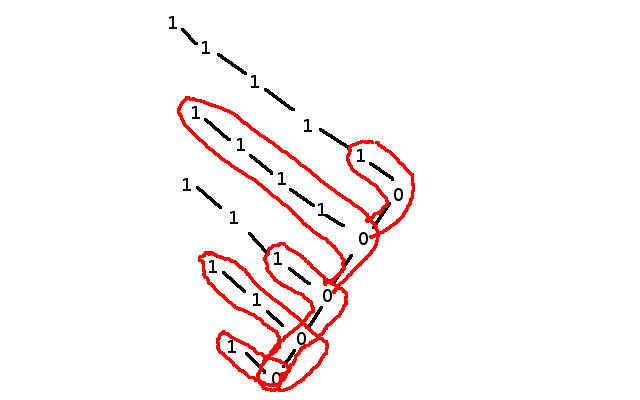
\includegraphics[scale=0.66]{entscheidbar.png}\\
Dabei besteht die Menge $0\ff W$ aus den rot-umrandeten W�rtern, also immer wenn $n\in A$ und $n\in \mathbb{N}$ dann kommt das echte Pr�fix in die Resultatmenge und wenn $n\in\mathbb{N}$ und $n\notin A$ dann kommt das ganze Wort rein, also:\\
$$0\ff W= \{0^{n+1} 1^{n+1} : n\in\mathbb{N} \wedge n\notin A\} \cup \{0^{n+1} 1: n\in \mathbb{N} \wedge n\in A\}$$
\textbf{Sollte} das soweit richtig sein so stelle ich fest, dass $n\notin A$ ja ein Problem ergibt da A nicht entscheidbar ist erfahre ich ja eigentlich nicht wenn $n\notin A$ ist ... soweit meine Gedanken dazu.
\end{document}
